% Chapter Template

\chapter{Theory} % Main chapter title
This chapter focuses on explaining the general theory behind the model and the methods used in this work.
Details regarding the exact problem definition, model adjustments, programs used and so on are given in
\hyperref[chap:methods]{Chapter \ref*{chap:methods}}.


\label{chap:theory} % Change X to a consecutive number; for referencing this chapter elsewhere, use \ref{ChapterX}

%----------------------------------------------------------------------------------------
%	SECTION 1
%----------------------------------------------------------------------------------------

\section{Compartmental modeling techniques}
Compartmental modeling revere to a modeling technique often used to systematically describe real world phenomena
like disease spreading\cite{compartementMod}. In these models the population is divided into different groups. 
Members of one group can move to another group. This movement is based on equations that are used to model the real
world behavior of each group. The following two sections introduce both the ``SIR'' and the ``SEIRD'' model. The
latter model was the focus on this work.

%-----------------------------------
%	SUBSECTION 1
%-----------------------------------
\subsection{Ordinary differential equations}

%-----------------------------------
%	SUBSECTION 2
%-----------------------------------
\subsection{Partial differential equations}


%-----------------------------------
%	SUBSECTION 3
%-----------------------------------
\subsection{The SIR model}
\label{sec:SIR}
In 1927 \cite{kermack1991contributions} first introduced their method to mathematically describe  
the course  of an infectious disease. The model divides a population into three distinct groups.

\begin{enumerate}[label=$\bullet$]
	\item \B{Susceptibles (S)}: Individuals that are naive to the infection and hence not immune. If in contact with
		the virus these individuals can migrate to the\linebreak ``Infected'' group
	\item \B{Infected (I)}: Individuals that are infected with the disease. Infected individuals contribute to the 
		infection of members of the susceptible group. At some point during their infection, these members
		transition to the ``Removed'' group.
	\item \B{Removed (R)}: Individuals that  have either overcome their infection and are now immune to the disease
		or have succumb to the disease and are diseased. They do not spread the virus and cannot be infected again.
\end{enumerate}

\par
The population changes of all three groups are described by mathematical equations\cite{mathSIR}. Notable variables
are the number of susceptible members (S), number of infected members (I), number of recovered members (R), $\alpha$
which is a positive constant that describes the transmission rate of the disease and $\beta$, which is a positive
constant between 0 and 1 that describes the transition rate (either recovery or death) between \B{I} and \B{R}.
$\beta$ can be rewritten as $\frac{1}{b}$, where $b$ is the average duration an infected individual remains contagious,
before it either recovers or dies. The model is illustrated in \hyperref[fig:SIR]{Figure \ref*{fig:SIR}}, the equations
are expressed as follows:

\begin{figure}
	\begin{center}
		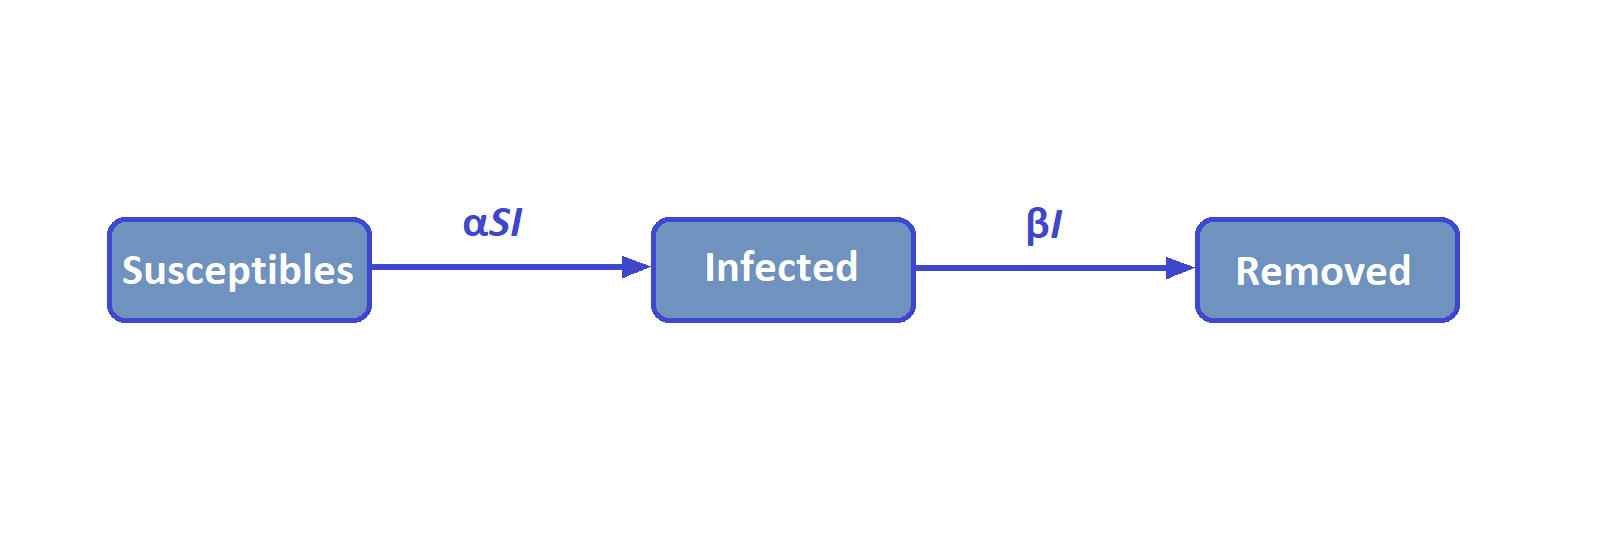
\includegraphics[width=0.75\textwidth]{./figures/SIR.png}
		\caption{Illustration of the population flow in the SIR model. S represents the ``Susceptible'', I
			the ``Infected'' and R the ``Removed'' population. The variable $\beta$ can also redefined
			as $\frac{1}{b}$, where $D$ is the average duration of contagiousness}
		\label{fig:SIR}
	\end{center}
\end{figure}


\begin{align}
	\label{eq:SIR1}
	\frac{dS}{dt} &= -\alpha S I \\
	\frac{dI}{dt} &= \alpha S I - \beta I \\
	\frac{dR}{dt} &= \beta I
\end{align}

\par
The model also assumes the total number of individuals in the system $N$ remains constant and that the sum of all transitions
between all three groups during every time step remains zero. This is expressed in the equations below.
$S(t)$, $I(t)$ and $R(t)$ express the number of individuals in each of the groups, at time $t$, respectively.

\begin{align}
	\label{eq:SIR2}
	I(t) + S(t) + R(t) &= N \\
	\frac{dS}{dt} + \frac{dI}{dt} + \frac{dR}{dt} = 0
\end{align}

\par
Since the model assumes, that the total population remains stable, phenomena like immigration or child birth are not accounted
for. This does not correctly represent the real world. However it is often assumed, that population fluctuations
due to these occurrences are minor enough compared to the entirety of a regions population, that they do not alter the results of the
simulation in a major way\cite{??}.\newline

\par
In order to correctly model the dynamics of an epidemic, the variables of these differential
equations (like $\alpha$ and $\beta$ in this case) must be determined correctly. This process is referred to as solving the equations.
Different techniques exist to do so. Two of these techniques are the \hyperref[sec:Gauss]{Gauss-Newton algorithm}\cite{Gauss??} and
\hyperref[sec:PSO]{Particle Swarm Optimization (PSO)}\cite{PSO??}. Both of these techniques will are explained in a later section.


%-----------------------------------
%	SUBSECTION 4
%-----------------------------------

\subsection{The SEIRD model}
\label{sec:SEIRD}
The SEIRD model is a variant of the simpler SIR model\cite{knodel20173d}
\textcolor{red}{(double check citation)}. % note
It introduces two new groups and describes the status for the infected population much more precise. The groups of the SEIRD
model are as follows:

\begin{enumerate}[label=$\bullet$]
	\item \B{Susceptibles (S)}: Individuals that are naive to the infection and hence not immune (identical to SIR).
	\item \B{Exposed (E)}: Individuals that are infected, but show no or very little symptoms. These individuals
		do not quarantine (yet) and are therefor contributing to the spread of the virus.
	\item \B{Infected (I)}: Individuals that have developed such a sever illness, that they need to be hospitalized.
	\item \B{Recovered (R)}: Individuals that  have overcome the infection and are now immune to the disease.
	\item \B{Diseased (D)}: Individuals that have succumb to the infection.
\end{enumerate}

\par
As described in the previous section, transition between the Individuals of different groups is a core
part of the model. The transition between the \B{S} and \B{E} population in SEIRD is equivalent to the transition
between \B{S} and \B{I} in SIR. However, the population outflow from the \B{E} group is split and can either move
to the \B{I} or to the \B{R} group. This allows the modeling of infections that result in quick recovery or an infection
with complications (defined by the hospitalization of the patient). The ratio between the two scenarios is governed by the variable
$\kappa$. In addition, the variable $q$ was introduced and now represents the average duration until recovery/hospitalization of an
infected individual. Similarly, the outflow of \B{I} is split between the populations of \B{R} and \B{D}. The ratio is governed
by the variable $\tau$. The equations for \B{R} and \B{D} were also adjusted to represent these changes. Lastly $D$ was redefined
as $p$, which now represents the average of a hospitalized individual to either recover or succumb to the infection.
\hyperref[fig:SEIRD]{Figure \ref*{fig:SEIRD}} illustrates all these changes. The modified equations are as follows:

\begin{align}
	\label{eq:SEIRD1}
	\frac{dS}{dt} &= -\alpha S E \\
	\frac{dE}{dt} &= \alpha S E -\frac{1}{q} E \\
	\frac{dI}{dt} &= \frac{\kappa}{q} E - \frac{1}{p} I \\
	\frac{dR}{dt} &= \frac{1-\kappa}{q} E + \frac{1-\tau}{p} I \\
	\frac{dD}{dt} &= \frac{\tau}{p} I
\end{align}


\begin{figure}
	\begin{center}
		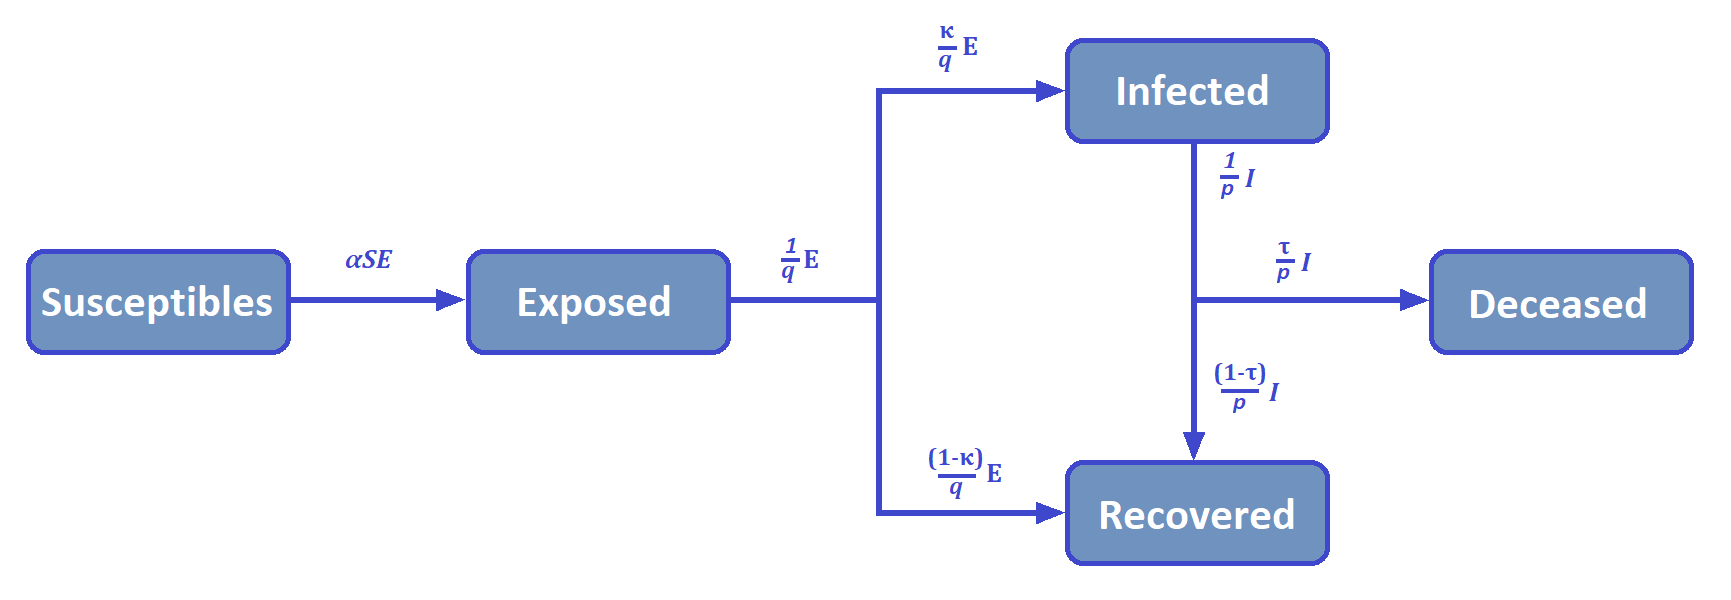
\includegraphics[width=0.75\textwidth]{./figures/SEIRD.png}
		\caption{Illustration of the population flow in the SEIRD model. S represents the ``Susceptible'', E the ``Exposed'',
			I the ``Infected'', R the ``Recovered'' and D the ``Diseased'' population. $\beta$ can also be expressed as
			$\frac{1}{\phi}$, where $\phi$ is the average time to recovery/hospitalization.}
		\label{fig:SEIRD}
	\end{center}
\end{figure}


\par
Like SIR, the SEIRD model assumes that the total number of individuals $N$ in the population remains constant during every step
of the modeling process. This leads to the equations expressed below. Again, $S(t)$, $E(t)$, $I(t)$, $R(t)$ and $D(t)$ are
expressing the number of individuals for each group at time $t$, respectively. $N$ remains the total number of individuals in the model.

\begin{align}
	\label{eq:SEIRD2}
	S(t) + E(t) + I(t) + R(t) + D(t) &= N \\
	\frac{dS}{dt} + \frac{dE}{dt}  + \frac{dI}{dt} + \frac{dR}{dt} + \frac{dD}{dt} = 0
\end{align}

\par
A model like this expresses the dynamics of an epidemic in much more detail. A weakness of the SIR model is that it does distinct between important
groups such as sick, but not infected and hospitalized individuals. The SEIRD model is capable of doing so and also allows for predicting
figures like the number of hospitalized individuals at time $t$.\newline

\par
This work focused mostly on the modeling capability of SIR in the transition stage between susceptibles and exposed. To better fulfill this
task, the model was redefined to accommodate for a lack of clear source data and to further refine the modeling of real wold phenomena. The changes
are described in detail in \hyperref[sec:SEIRDredef]{chapter~\ref*{chap:methods}, section~\ref*{sec:SEIRDredef}}.



%----------------------------------------------------------------------------------------
%	SECTION 2
%----------------------------------------------------------------------------------------

\section{Variable optimization algorithms}
In order for the presented models to work properly, it is important to determine the correct value for each unknown variable. There are many
methods to determine these variables. In the context of differential equations this process is often referred to as ``solving'' the equations.
Algorithms and methods that try to achieve this are generally referred to as ``solvers''.\newline

\par
The following sections will explain two methods used in this work. The Gauss-Newton algorithm and the Particle Swarm Optimization algorithm (PSO).

%-----------------------------------
%	SUBSECTION 1
%-----------------------------------

\subsection{Gauss-Newton algorithm}
\label{sec:Gauss}

%-----------------------------------
%	SUBSECTION 2
%-----------------------------------

\subsection{Particle Swarm Optimization}
\label{sec:PSO}





%----------------------------------------------------------------------------------------
%	SECTION 3
%----------------------------------------------------------------------------------------

\section{Data post processing}

\subsection{box plots}

